\documentclass[10pt, xcolor={dvipsnames}]{beamer}
\usetheme{Boadilla}

\setbeamerfont{title}{series=\bfseries}
\setbeamerfont{author}{series=\normalfont}
\setbeamerfont{frametitle}{series=\bfseries}
\setbeamerfont{footline}{series=\bfseries}
\setbeamertemplate{caption}[numbered]
\usepackage{caption}

\definecolor{links}{HTML}{2A1B81}
\hypersetup{colorlinks,linkcolor=,urlcolor=links}
\setbeamercolor{bibliography item}{fg=black}
\setbeamercolor{bibliography entry author}{fg=black}
\setbeamercolor{bibliography entry title}{fg=black}
\setbeamercolor{bibliography entry location}{fg=black}
\setbeamercolor{bibliography entry note}{fg=black}

\usepackage[utf8x]{inputenc}
\usepackage[english]{babel}

\usepackage{graphicx}


%----------------------------------------------------------------------------------------
%	TITLE PAGE
%----------------------------------------------------------------------------------------

\setbeamerfont{title}{size=\large}
\setbeamerfont{author}{size=\normalsize}
\setbeamerfont{date}{size=\footnotesize}

\title[Longevity Research Screening]{A Simple Machine Learning Framework to Aid Citation Screening in Systematic Reviews and Meta-Analyses of Aging and Longevity Research Studies}
\author[\textcolor{white}{Marko Lalović}]{\textcolor{black}{Marko Lalović}}
\date[\textcolor{white}{\today}]{\textcolor{black}{\today}}

\defbeamertemplate*{title page}{customized}[1][]
{
  \usebeamerfont{title}\inserttitle\par
  \usebeamerfont{subtitle}\usebeamercolor[fg]{subtitle}\insertsubtitle\par
  \bigskip
  \usebeamerfont{author}\insertauthor\par
  \usebeamerfont{institute}\insertinstitute\par
  \usebeamerfont{date}\insertdate\par
  \usebeamercolor[fg]{titlegraphic}\inserttitlegraphic
  \bigskip
}


\begin{document}
\begin{frame}
\begin{center}
\maketitle
\begin{figure}
    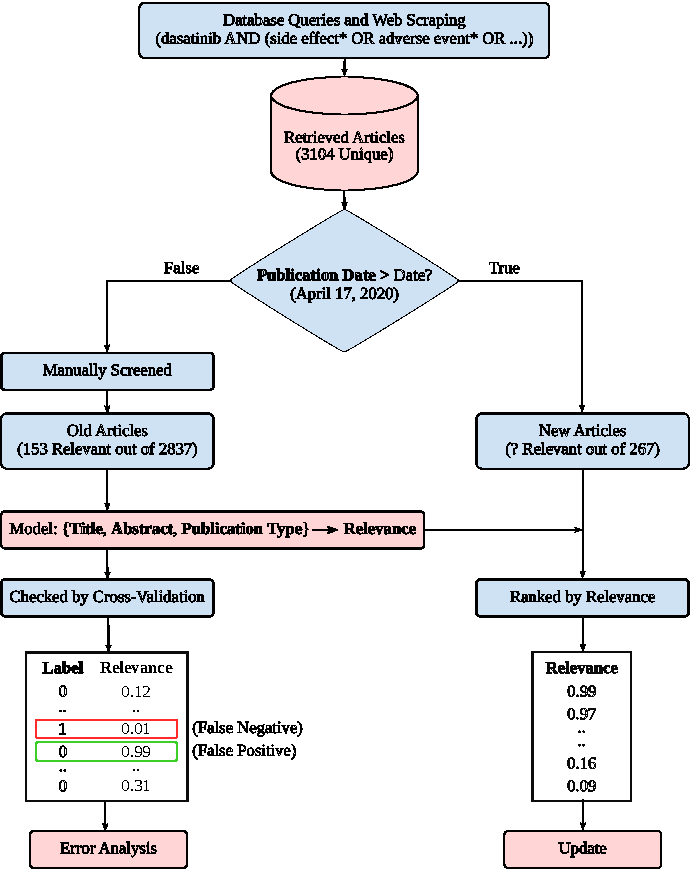
\includegraphics[width=\linewidth]{../report/diagrams/general-overview/general-overview-crop.pdf}
    \caption{General overview of proposed framework.}
\end{figure}    
\end{center}
\end{frame}


%----------------------------------------------------------------------------------------
%	PRESENTATION SLIDES
%----------------------------------------------------------------------------------------

\section{Background}
\begin{frame}
\frametitle{Background}
\begin{itemize}
\item A systematic review typically addresses a specific clinical question by collecting and analyzing data from all the relevant and unbiased set of studies. 
\item Citation screening is the first yet tedious task of narrowing down the large set of citations retrieved via a broad database query to those relevant for the review.
\end{itemize}
\end{frame}

\begin{frame}
\frametitle{Idea}
Develop a machine learning framework to semi-automate citation screening in systematic reviews and meta-analyses, thereby reducing reviewers workload (and screening errors).
\end{frame}

\begin{frame}
\frametitle{Related Work}
\begin{itemize}
\item Wallace et al. developed a semi-automated citation screening algorithm
for systematic reviews of biomedical literature. 
\item Bannach-Brown et al. described their approaches to aid citation
screening for a systematic review of pre-clinical animal studies. 
\item Howard et al. deployed a general software system that automate the required methodologies called ``SWIFT-Review". 
\item Przybyła et.al introduced a web-based software system called ``RobotAnalyst". \item O'Mara-Eves et al. performed a systematic review of current approaches.
\item To date, no use of any tools related to automating (or semi-automating) the screening process of systematic reviews or meta-analyses of aging and longevity research was reported.
\end{itemize}
\end{frame}

\begin{frame}
\frametitle{Our Contribution}
\begin{itemize}
\item Present a simple machine learning framework that can be used in the screening stage of systematic reviews or meta-analyses of aging and longevity research studies.
\item Present our experimental results on dataset related to \href{https://brain.forever-healthy.org/display/EN/}{Dasatinib and Quercetin Senolytic Therapy Risk-Benefit Analysis}\footnotemark (D\&Q Analysis).
\end{itemize}
\footnotetext[1]{The analysis is part of ``Rejuvenation Now" non-profit initiative that: ``seeks to continuously identify potential rejuvenation therapies and systematically evaluate their risks, benefits, and associated therapeutic protocols to create transparency" published by Forever Healthy Foundation.}%
\end{frame}

\section{Methods}
\begin{frame}
\frametitle{Outline}
\begin{figure}[H]
\centering
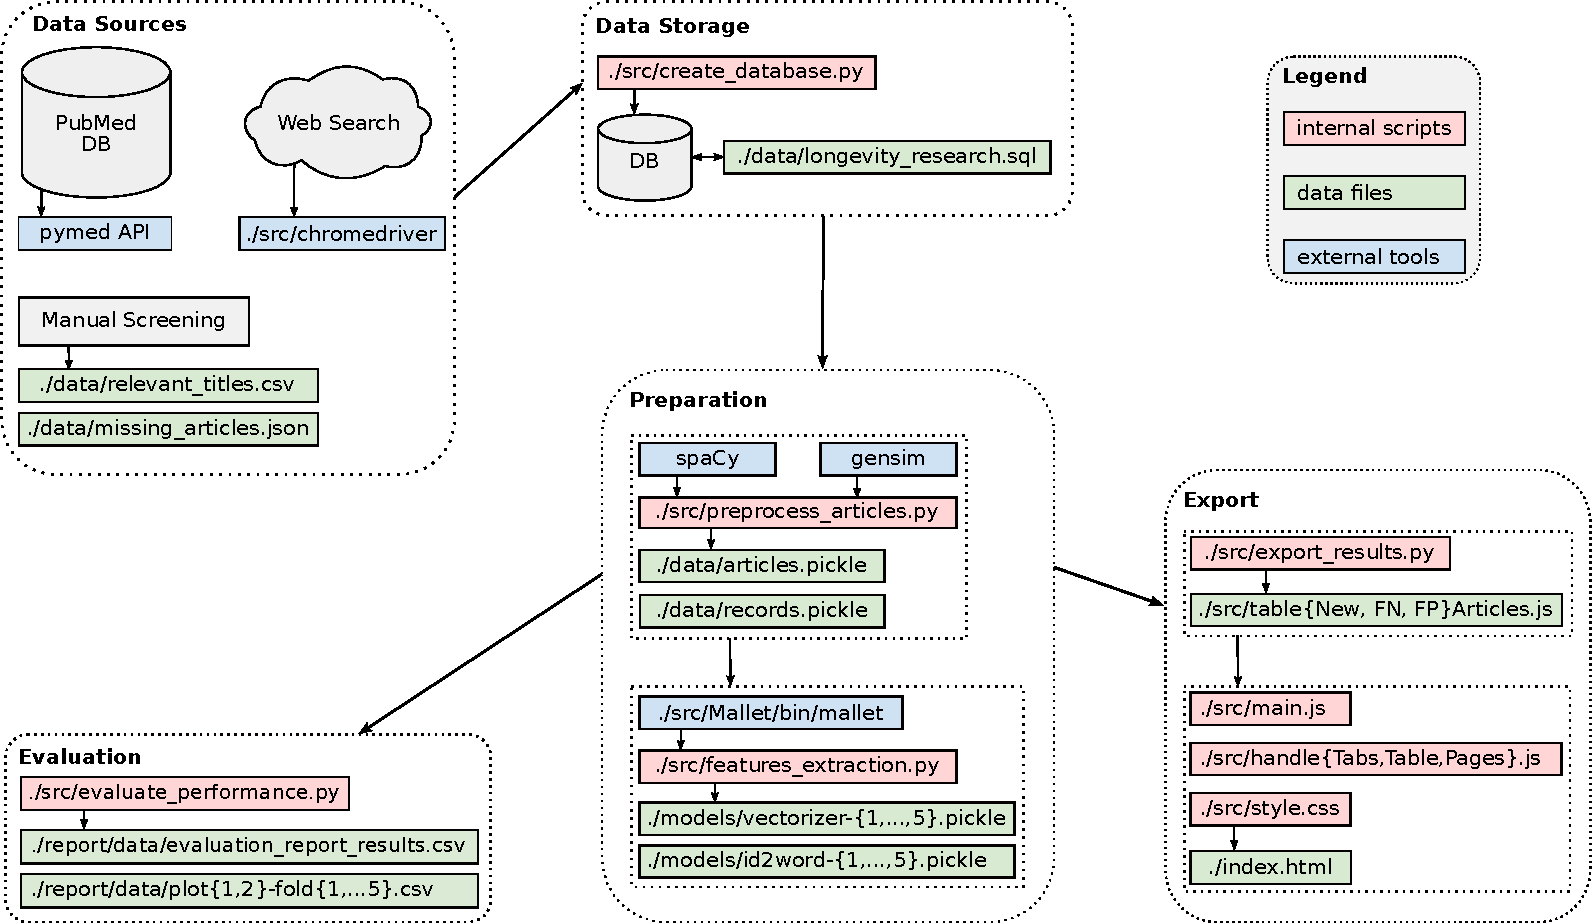
\includegraphics[width=1\textwidth]{../report/diagrams/technical-overview/technical-overview-crop.pdf}
\caption{Technical Overview.}
\end{figure}
\end{frame}

\begin{frame}
\frametitle{Features}
Extracted features are based on:
\begin{itemize}
\item Provided list of search terms: dasatinib, senolytic, senescent, ...
\item Possible publication types: case report, clinical trial, review, ...
\item TF-IDF scores of terms: chronic myeloid, adverse event, tyrosine kinase, ...
\item LDA model probabilities of belonging to topics: \\
\end{itemize}
\vspace{1mm}
\centering
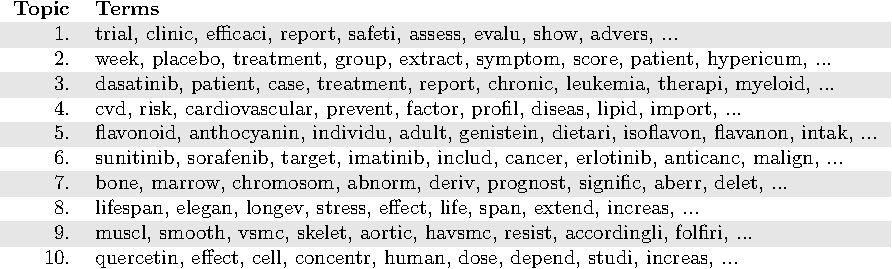
\includegraphics[width=1\textwidth]{../report/tables/topics/topics-crop.pdf}
...
\end{frame}

\begin{frame}
\frametitle{Model}
\begin{itemize}
\item Used L1 regularized logistic regression model from scikit-learn.
\item Fitted using Liblinear solver with balanced class weights. 
\item Placed more emphasis on recall by using recall scorer.
\end{itemize}
\begin{definition}[Relevance]
The model estimates the conditional probability, called {\it relevance score}, that a given document $d$ is relevant given feature vector $X^{d}$:
$$
\text{Pr}(\text{$d$ is relevant} | X^{d})
$$
\end{definition}
\end{frame}

\begin{frame}
\frametitle{Threshold Selection}
The selected cut-off threshold for D\&Q Analysis was 0.26 where the binary classifier achieved 95\% recall:

\begin{figure}[H]
\centering
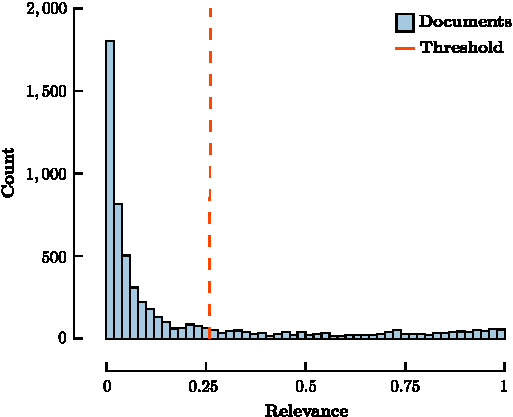
\includegraphics[width=0.7\textwidth]{../report/figures/threshold-selection/threshold-selection-crop.pdf}
\end{figure}
\end{frame}

\begin{frame}
\frametitle{Errors}
There are four possible outcomes of comparing the classification result with human assigned label:
\begin{figure}[H]
\centering
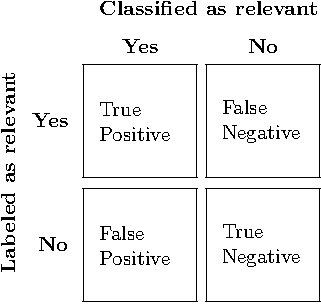
\includegraphics[width=0.4\textwidth]{../report/tables/confusion-matrix/confusion-matrix-crop.pdf}
\end{figure}
\end{frame}

\begin{frame}
\frametitle{Performance Evaluation}
Performance was assessed by:
\begin{definition}[Statistical measures]
{\it Precision} $P$ is the fraction of documents labeled as relevant among documents classified as relevant:
$$
P = \frac{TP}{TP + FP}
$$
{\it Recall} $R$ (also known as {\it sensitivity}) is the fraction of documents labeled as relevant that were also classified as relevant:
$$
R = \frac{TP}{TP + FN}
$$
{\it Work Saved over Sampling} $WSS@R$ is the reduction of documents that need to be screened compared to a random ordering of the documents to achieve a level of recall $R$:

$$
WSS@R = \frac{TN + FN}{N} - (1 - R)
$$
\end{definition}
\end{frame}

\section{Results}
\begin{frame}
\frametitle{Evaluation Results}
\begin{table}
\centering
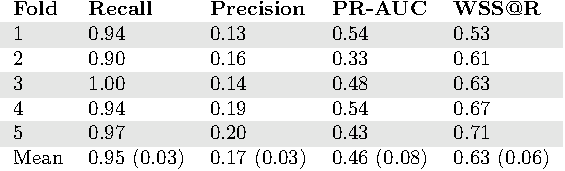
\includegraphics[width=.8\textwidth]{../report/tables/evaluation-results/evaluation-results-crop.pdf}
\caption{Summarized results of 5-fold cross-validation for D\&Q Analysis}
\end{table}
\end{frame}

\begin{frame}
\frametitle{Evaluation of Results}
\begin{figure}
\centering
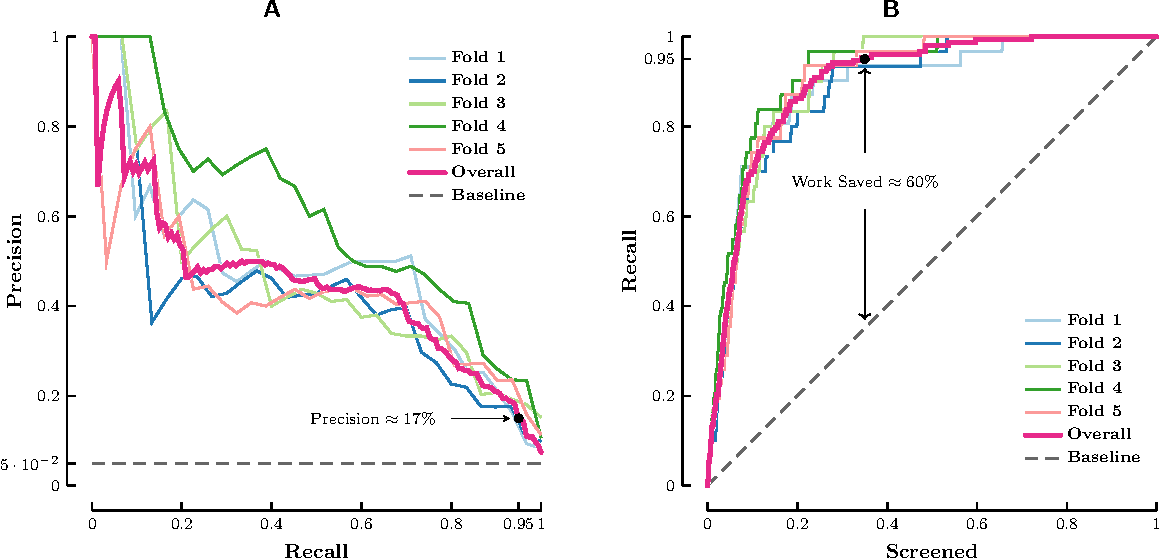
\includegraphics[width=1\textwidth]{../report/figures/performance-evaluation/combined/performance-evaluation-crop.pdf}
\caption{Visualized results of 5-fold cross-validation for D\&Q Analysis}
\end{figure}
\end{frame}

\begin{frame}
\frametitle{Export}
\begin{figure}
\centering
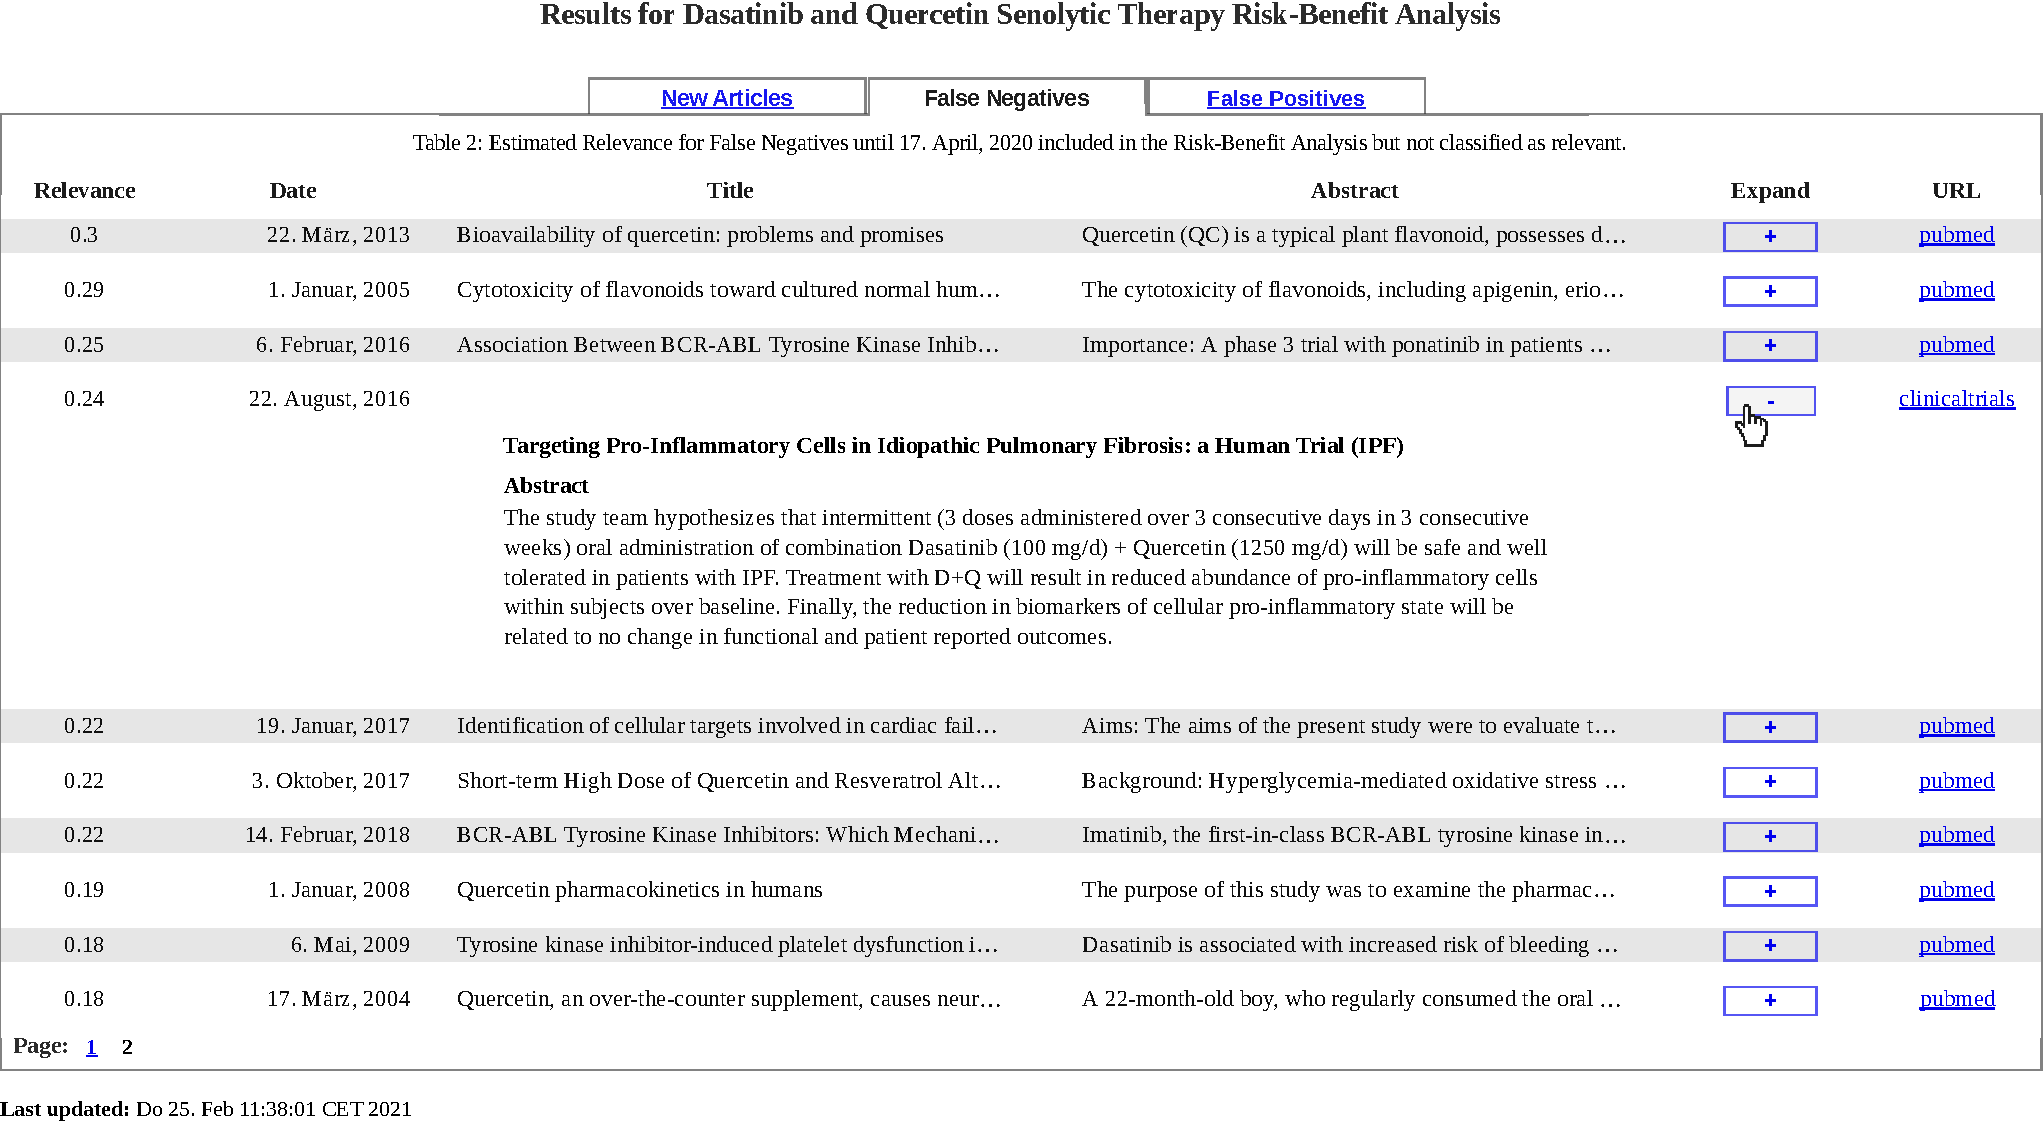
\includegraphics[width=1\textwidth]{../report/tables/export-tables/export-tables-crop.pdf}
\caption{Interactive tables of exported documents for D\&Q Analysis.}
\label{fig:export}
\end{figure}
\end{frame}

\begin{frame}
\frametitle{Links}
\begin{itemize}
\item Interactive tables of exported documents for D\&Q Analysis: \url{https://markolalovic.com/longevity-research-screening/}
\item Technical report: \url{https://zenodo.org/record/4593957/files/zenodo.4593957.pdf}
\item Source code: \url{https://github.com/markolalovic/longevity-research-screening/}
\end{itemize}
\end{frame}

\begin{frame}
\frametitle{References}
\scalebox{0.9}{\begin{minipage}{1.20\textwidth}
\begin{thebibliography}{5}
\bibitem{1} Bannach-Brown, A., Przybyła, P., Thomas, J. et al. ``Machine learning algorithms for systematic review: reducing workload in a preclinical review of animal studies and reducing human screening error.", Syst Rev 8, 23 (2019). \url{https://doi.org/10.1186/s13643-019-0942-7}
\bibitem{2} Howard BE, Phillips J, Miller K, et al. ``SWIFT-Review: a text-mining workbench for systematic review.", Syst Rev. 2016;5:87. Published 2016 May 23. \url{doi:10.1186/s13643-016-0263-z}
\bibitem{3} O’Mara-Eves, A., Thomas, J., McNaught, J. et al. ``Using text mining for study identification in systematic reviews: a systematic review of current approaches.", Syst Rev 4, 5 (2015). \url{https://doi.org/10.1186/2046-4053-4-5}
\bibitem{4} Przybyła P, Brockmeier AJ, Kontonatsios G, et al. ``Prioritising references for systematic reviews with RobotAnalyst: A user study.", Res Synth Methods. 2018;9(3):470-488. \url{https://doi.org/10.1002/jrsm.1311}
\bibitem{5} Wallace, B.C., Trikalinos, T.A., Lau, J. et al. ``Semi-automated screening of biomedical citations for systematic reviews.", BMC Bioinformatics 11, 55 (2010). \url{https://doi.org/10.1186/1471-2105-11-55}
\end{thebibliography}
\end{minipage}}
\end{frame}
\end{document} 
